% Tags: 4321102, multiplexer, working, decoder
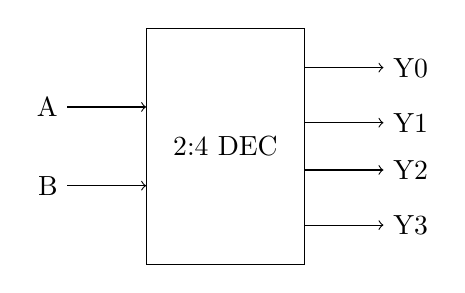
\begin{tikzpicture}
    \node[draw, minimum width=2cm, minimum height=3cm] (dec) {2:4 DEC};
    \draw[<-] (dec.west) ++(0,0.5) -- ++(-1,0) node[left] {A};
    \draw[<-] (dec.west) ++(0,-0.5) -- ++(-1,0) node[left] {B};
    
    \draw[->] (dec.east) ++(0,1.0) -- ++(1,0) node[right] {Y0};
    \draw[->] (dec.east) ++(0,0.3) -- ++(1,0) node[right] {Y1};
    \draw[->] (dec.east) ++(0,-0.3) -- ++(1,0) node[right] {Y2};
    \draw[->] (dec.east) ++(0,-1.0) -- ++(1,0) node[right] {Y3};
\end{tikzpicture}
